\documentclass[preprint2]{aastex62}

\bibliographystyle{aasjournal}
\usepackage{graphicx}
\usepackage[suffix=]{epstopdf}
\usepackage{natbib}
\usepackage{amsmath}
\usepackage{url}
\usepackage{xspace}

%    Make Scientific Notation
\providecommand{\e}[1]{\ensuremath{\times 10^{#1}}}

% make the word Kepler italicized
\newcommand{\Kepler}{\textsl{Kepler}\xspace}



\begin{document}
%%%%%%%%%%%%%%%%%%%%%%
\title{Rotating Stars from \Kepler Observed with Gaia DR2}

\shorttitle{Rotating Stars}
\shortauthors{Davenport et al.}


\correspondingauthor{James. R. A. Davenport}
\email{James.Davenport@wwu.edu}

\author{James. R. A. Davenport}
\altaffiliation{NSF Astronomy and Astrophysics Postdoctoral Fellow}
\altaffiliation{DIRAC Fellow}
\affiliation{Department of Physics \& Astronomy, Western Washington University, 516 High St., Bellingham, WA 98225, USA}
\affiliation{Department of Astronomy, University of Washington, Seattle, WA 98195, USA}


\author{Kevin R. Covey}
\affiliation{Department of Physics \& Astronomy, Western Washington University, 516 High St., Bellingham, WA 98225, USA}


 
 

%%%%%%%%%%%%%%%%%%%%%%%%%%%%%%
\begin{abstract}
Astrometric data from the recent Gaia Data Release 2 has been matched against the sample of stars from \Kepler with known rotation periods. 
\end{abstract}



%%%%%%%%%%%%%%%%%%%%%%%%%%%%%%
\section{Introduction}

The \Kepler mission \citep{borucki2010} 





\citet{mcquillan2013} bimodal period distribution 
\citep{mcquillan2014}.

\citet{davenport2017} looked at this with Gaia DR1, extending period gap to G dwarfs, pointing to SFH as cause. sub giant contamination was the thing. Now we can finally follow up on this and study the full \Kepler rotation period sample

 \citep{gaia} mission 
 


In this letter




%%%%%%%%%%%%%%%%%%%%%%
\section{The \Kepler--Gaia Data}
%Rotation periods in this study come from \citet{mcquillan2014}, who performed an Auto-Correlation Function analysis of \Kepler stars cooler than 6500 K that had at least $\sim$2 years of observation. The periods recovered from this approach generally agree very well with those found via Lomb-Scargle Periodograms \citep[e.g.][]{reinhold2013,aigrain2015}. Sources with multiple distinct periods, such as from binary systems with two spotted stars \citep[e.g.][]{lurie2015} are detected by \citet{mcquillan2014}, but are not included in the following analysis.

%The Gaia Data Release 1 (DR1) provides astrometric positions for over $10^9$ sources from the first year of observation with Gaia. The Tycho-Gaia Astrometric Solution (TGAS) measures improved proper motions and parallaxes for 2 million nearby, bright sources by extending the astrometric solutions from Tycho and Hipparcos. While the TGAS data are not a complete astrometric survey, and have possible systematics in the reported parallaxes \citep{gaia_dr1,stassun2016}, they represent a significant improvement in the astrometry and kinematics available for stars in the \Kepler field.


data xmatched by M. Bedell between Kepler DR25 (CITE) and Gaia DR2 (CITE), using 1arcsec radius.
distances using the updated prescription from \citet{bailer-jones2018}




%%%%%%%%%%%%%%%%%%%%%%
\section{Selecting Main Sequence Stars}



\begin{figure*}[]
\centering
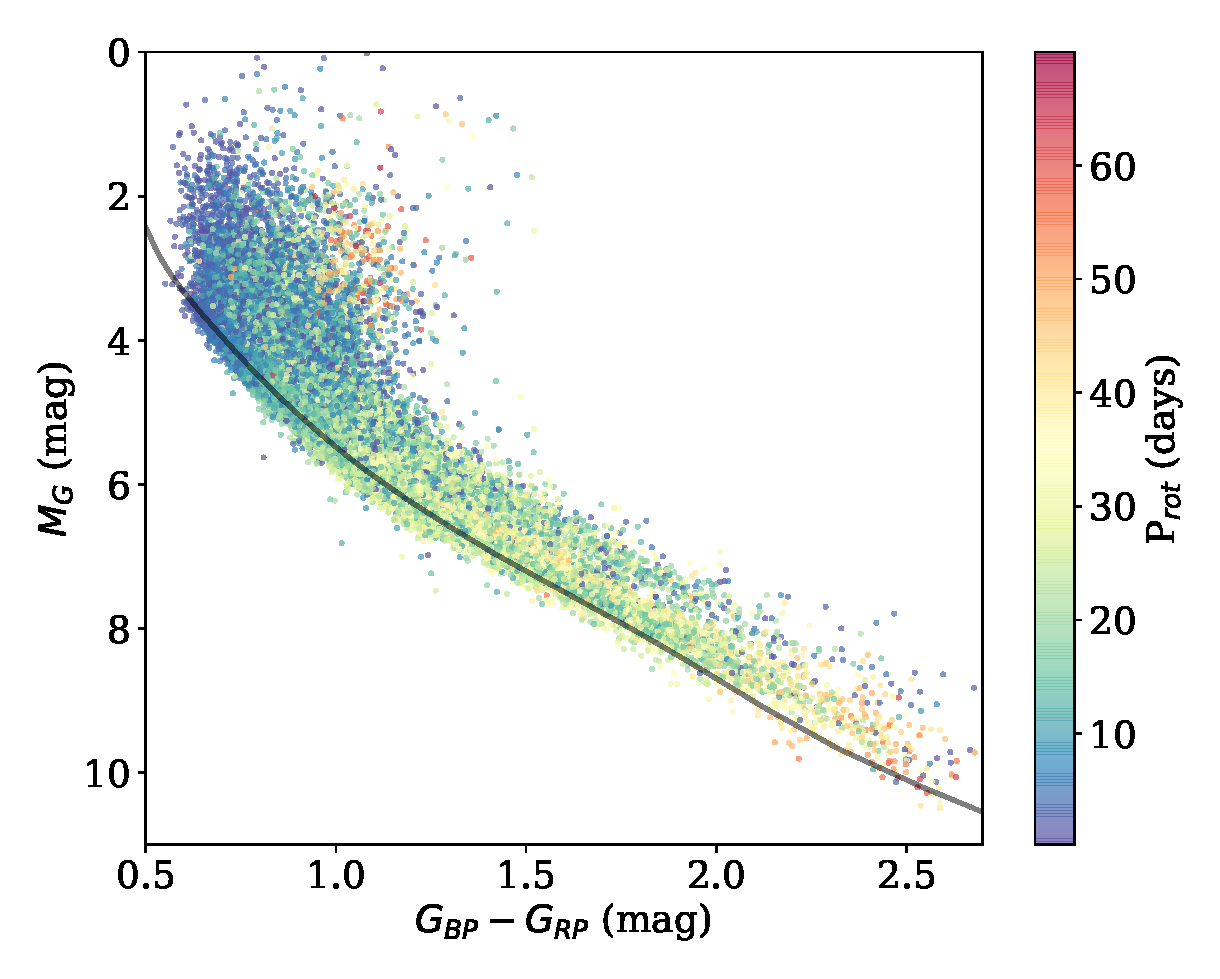
\includegraphics[width=6in]{../figures/cmd}
\caption{
Color--magnitude diagram for 30,305 \Kepler stars from the \citet{mcquillan2014} sample that are included in Gaia DR2, colored by their measured rotation period. For reference we show a $10^9$ year MIST isochrone (black line) used to select likely main sequence, single stars (black line). A track of binary  stars is apparent $\sim$0.7 mag above the main sequence. As in \citet{davenport2017}, we find significant contamination of the rotation period sample for bluer stars by sub-giants.}
\label{fig:cmd}
\end{figure*}





%Though \citet{mcquillan2014} attempted to only measure periods for dwarf stars, the sample of \Kepler--Gaia matched stars contains both main sequence dwarfs and evolved stars (giants and subgiants). Previous studies have shown  significant contamination by giants or subgiants can affect the implied variability properties of dwarf stars \citep{ciardi2011,mann2012}. Therefore to properly understand the nature of the period distribution and its implications for age-dating field stars, a robust sample of main sequence stars must be selected.
%
%Faint stars were removed by requiring sources have $G$-band flux errors $<1$\%. To ensure accurate distances, and therefore luminosities, parallaxes were required to have errors $<0.4$ mas. These cuts left a total of 894 stars from the \Kepler--TGAS matched sample (68\%). The Hertzsprung--Russell (HR) diagram for these stars is shown in Figure \ref{fig:HR}, with each point colored by its \Kepler-measured rotation period. Example isochrones from the \citet{bressan2012} grid are shown for two ages. A systematic offset of $\sim$0.5 magnitudes is found between the measured absolute $G$-band and the isochrone's main sequence. This offset is likely due to calibration differences between the nominal and actual $G$-band (A. Brown, private communication).
%
%
%The HR-period diagram in Figure \ref{fig:HR} shows stars with a range of evolutionary states, and could help test post-main sequence angular momentum evolution models \citep[e.g.][]{donascimento2012}. Outliers in this diagram are either due to erroneous cross-matching in the \Kepler and Gaia catalogs, or represent interesting systems such as rare binary star configurations or stars that have undergone mergers or ingested giant planets \citep{massarotti2008,tayar2015}. For example, examining the 2 Micron All Sky Survey \citep[2MASS][]{2mass} image on SIMBAD for 
%the rapidly rotating star at $T_{eff}=4500$ K, $M_G=4.5$ mag, $P_{rot}$=0.652 d, in Figure \ref{fig:HR} (KIC 07957709), this source appears highly contaminated with three point sources clustered within $\sim$10 arcseconds, likely leading to an erroneous position in the HR diagram, and possibly incorrect variability measurements with \Kepler.
%Investigating all such outliers in Figure \ref{fig:HR} is beyond the scope of this work, but these targets are worth further study as they may reveal new physics.
%
%
%
%Main sequence stars were selected using a simple cut around 300 Myr isochrone. Given the systematic offset of $\sim$0.5 mag between the Myr isochrone and the observed $M_G$ values, a fairly wide band of stars ($0\le \Delta M_G \le 1$) was selected as being ``close to the main sequence''. The final sample included 440 stars. This simplistic cut is not a robust dwarf--giant, nor single--binary star separator, but serves to select a sample of mostly main sequence stars for the illustrative purpose of this work. More precise selection will require an improved isochrone track, as well as updated parallaxes from the full Gaia DR2.
%



%%%%%%%%%%%%%%%%%%%%%%%
%\section{Extending the Spin-Down Gap}
%A bimodal period distribution was first discovered by \citet{mcquillan2013} for \Kepler M dwarfs, who found a dearth of objects with periods around $\sim$25 days. Follow-up work by \citet{mcquillan2014} found this bimodality extended to K dwarfs, up to $T_{eff}\sim5500$. Figure \ref{fig:gyro} shows the rotation period distribution for the final 440 star sample of likely main sequence stars. The bimodality appears to extend smoothly through to the hottest stars in this sample. 
%
%While these periods for field stars were robustly measured by \citet{mcquillan2014} and others, the bimodality did not appear in previous \Kepler work due to the high contamination rate by subgiants for these bluer, hotter stars.  414 rotating stars had acceptable photometric and parallax uncertainties in TGAS, but were culled from this sample for having $M_G$ luminosities higher than the main sequence cut in \S3 above. Note that distributions of $\log g$ values from the Kepler Input Catalog \citep{brown2011a} for both the main sequence and subgiant stars were not statistically different.






\begin{figure*}[]
\centering
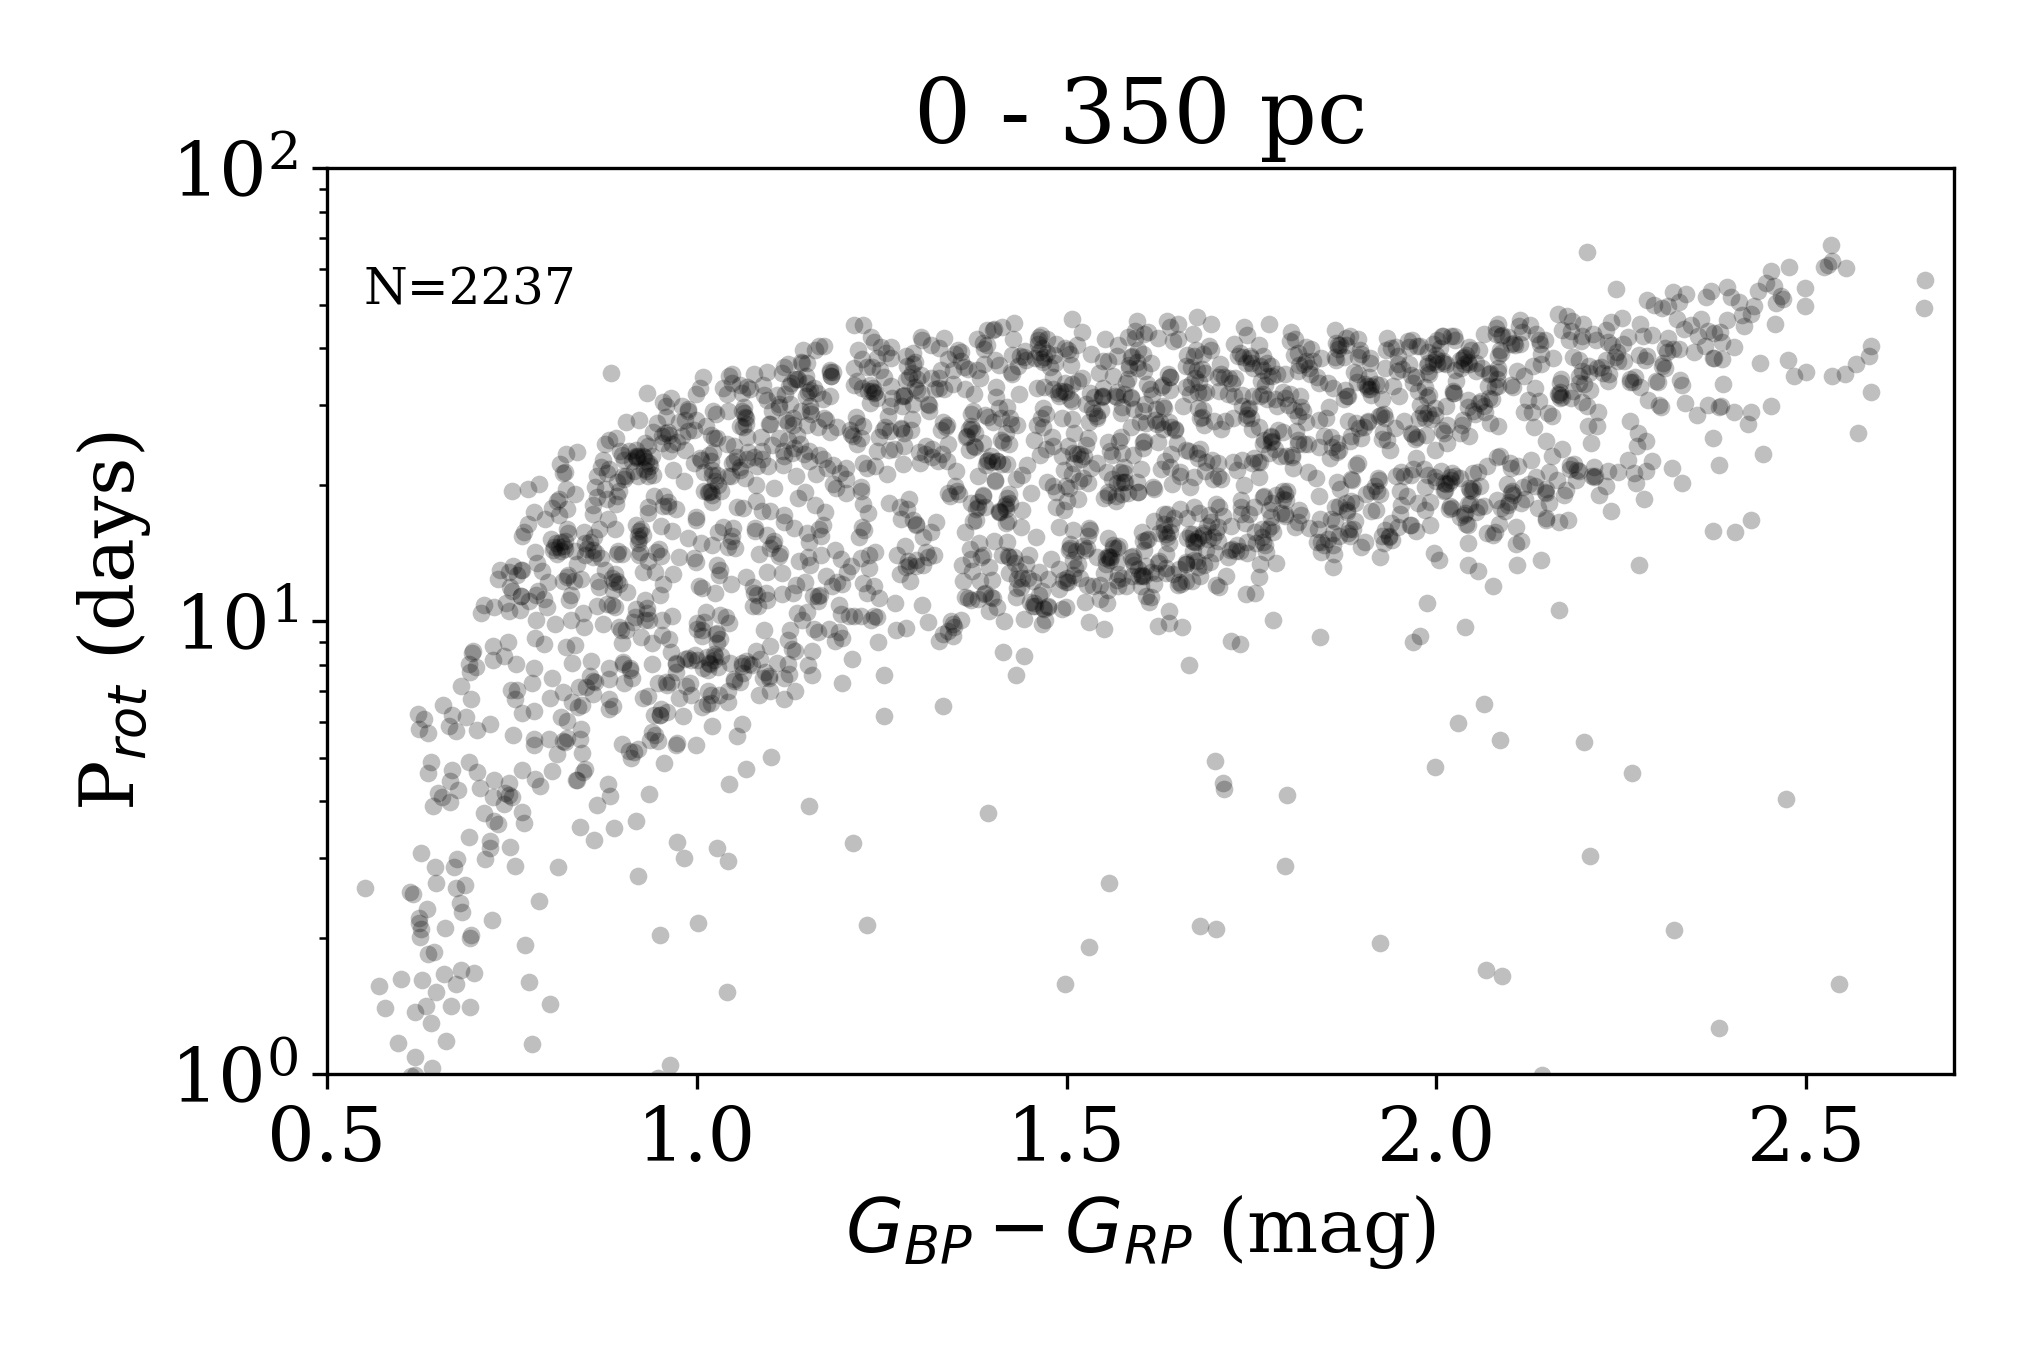
\includegraphics[width=3.5in]{../figures/rot_dist_0}
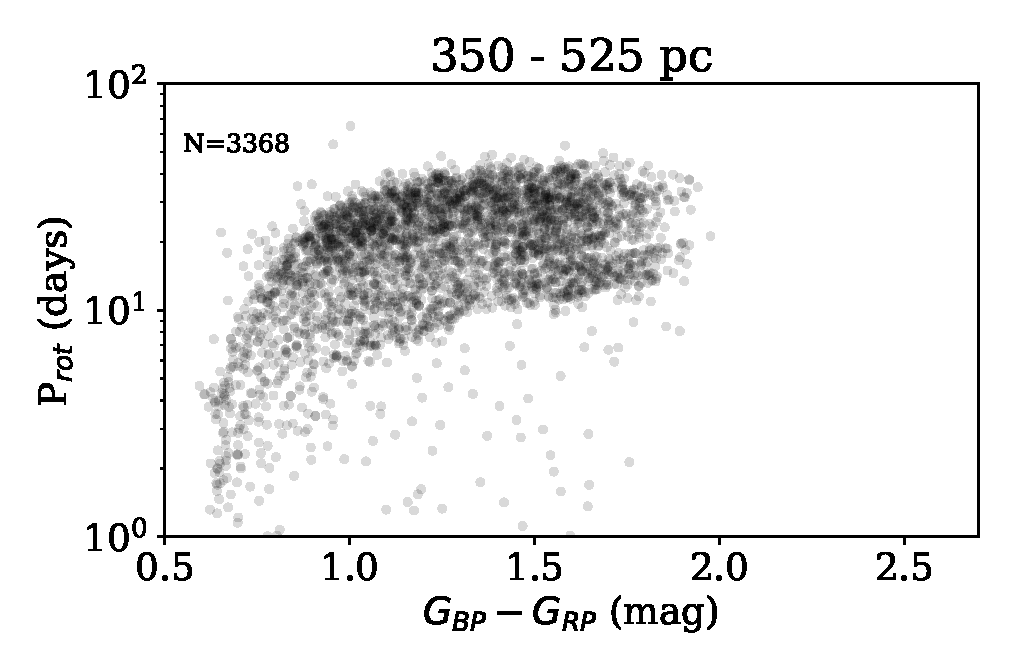
\includegraphics[width=3.5in]{../figures/rot_dist_350}
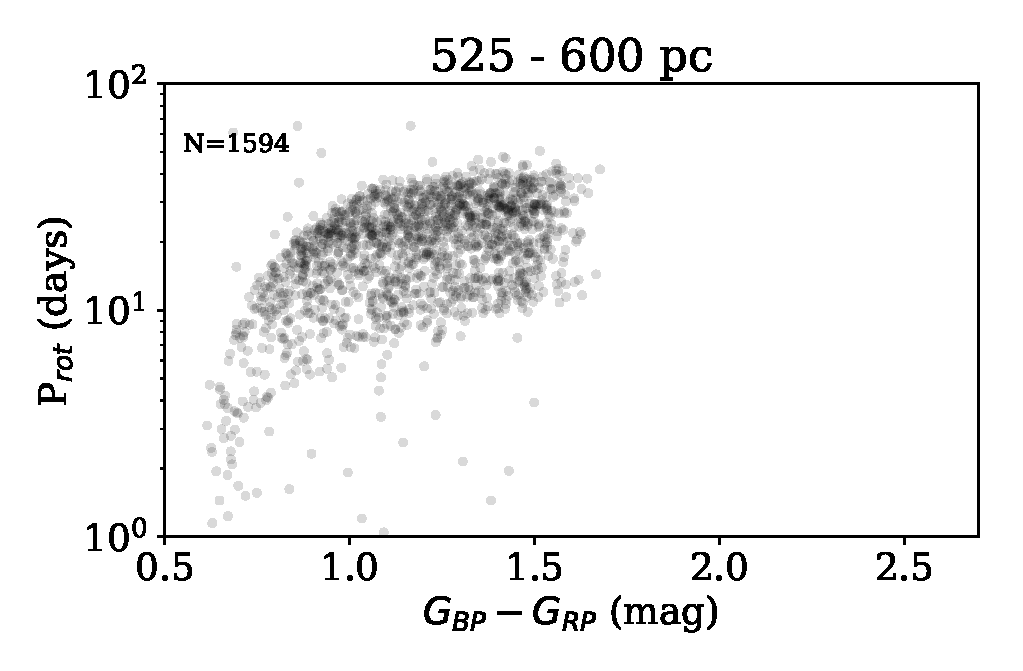
\includegraphics[width=3.5in]{../figures/rot_dist_525}
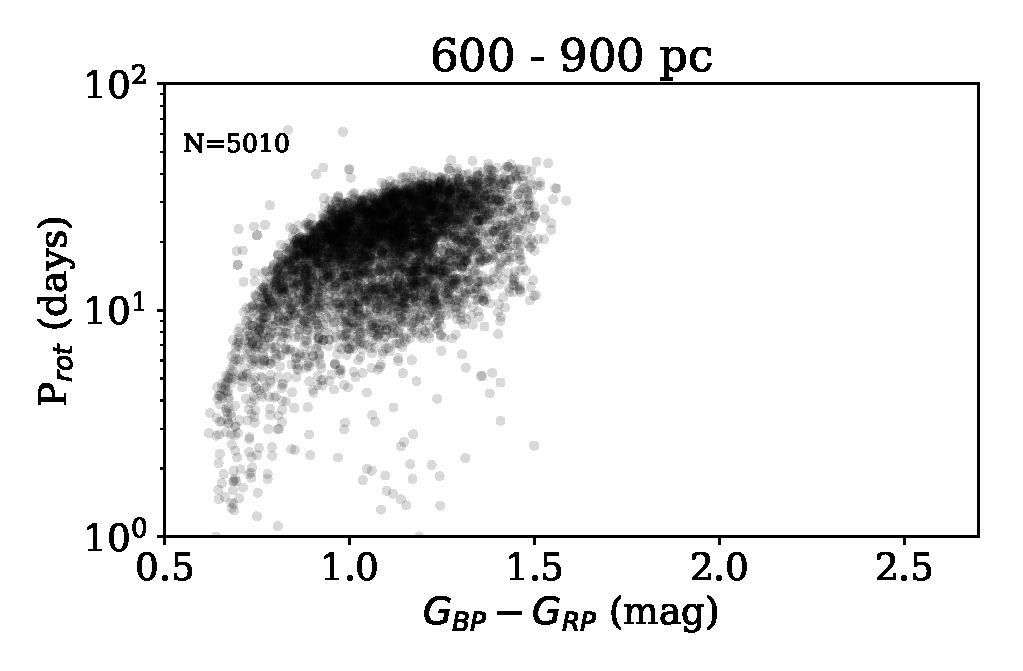
\includegraphics[width=3.5in]{../figures/rot_dist_600}
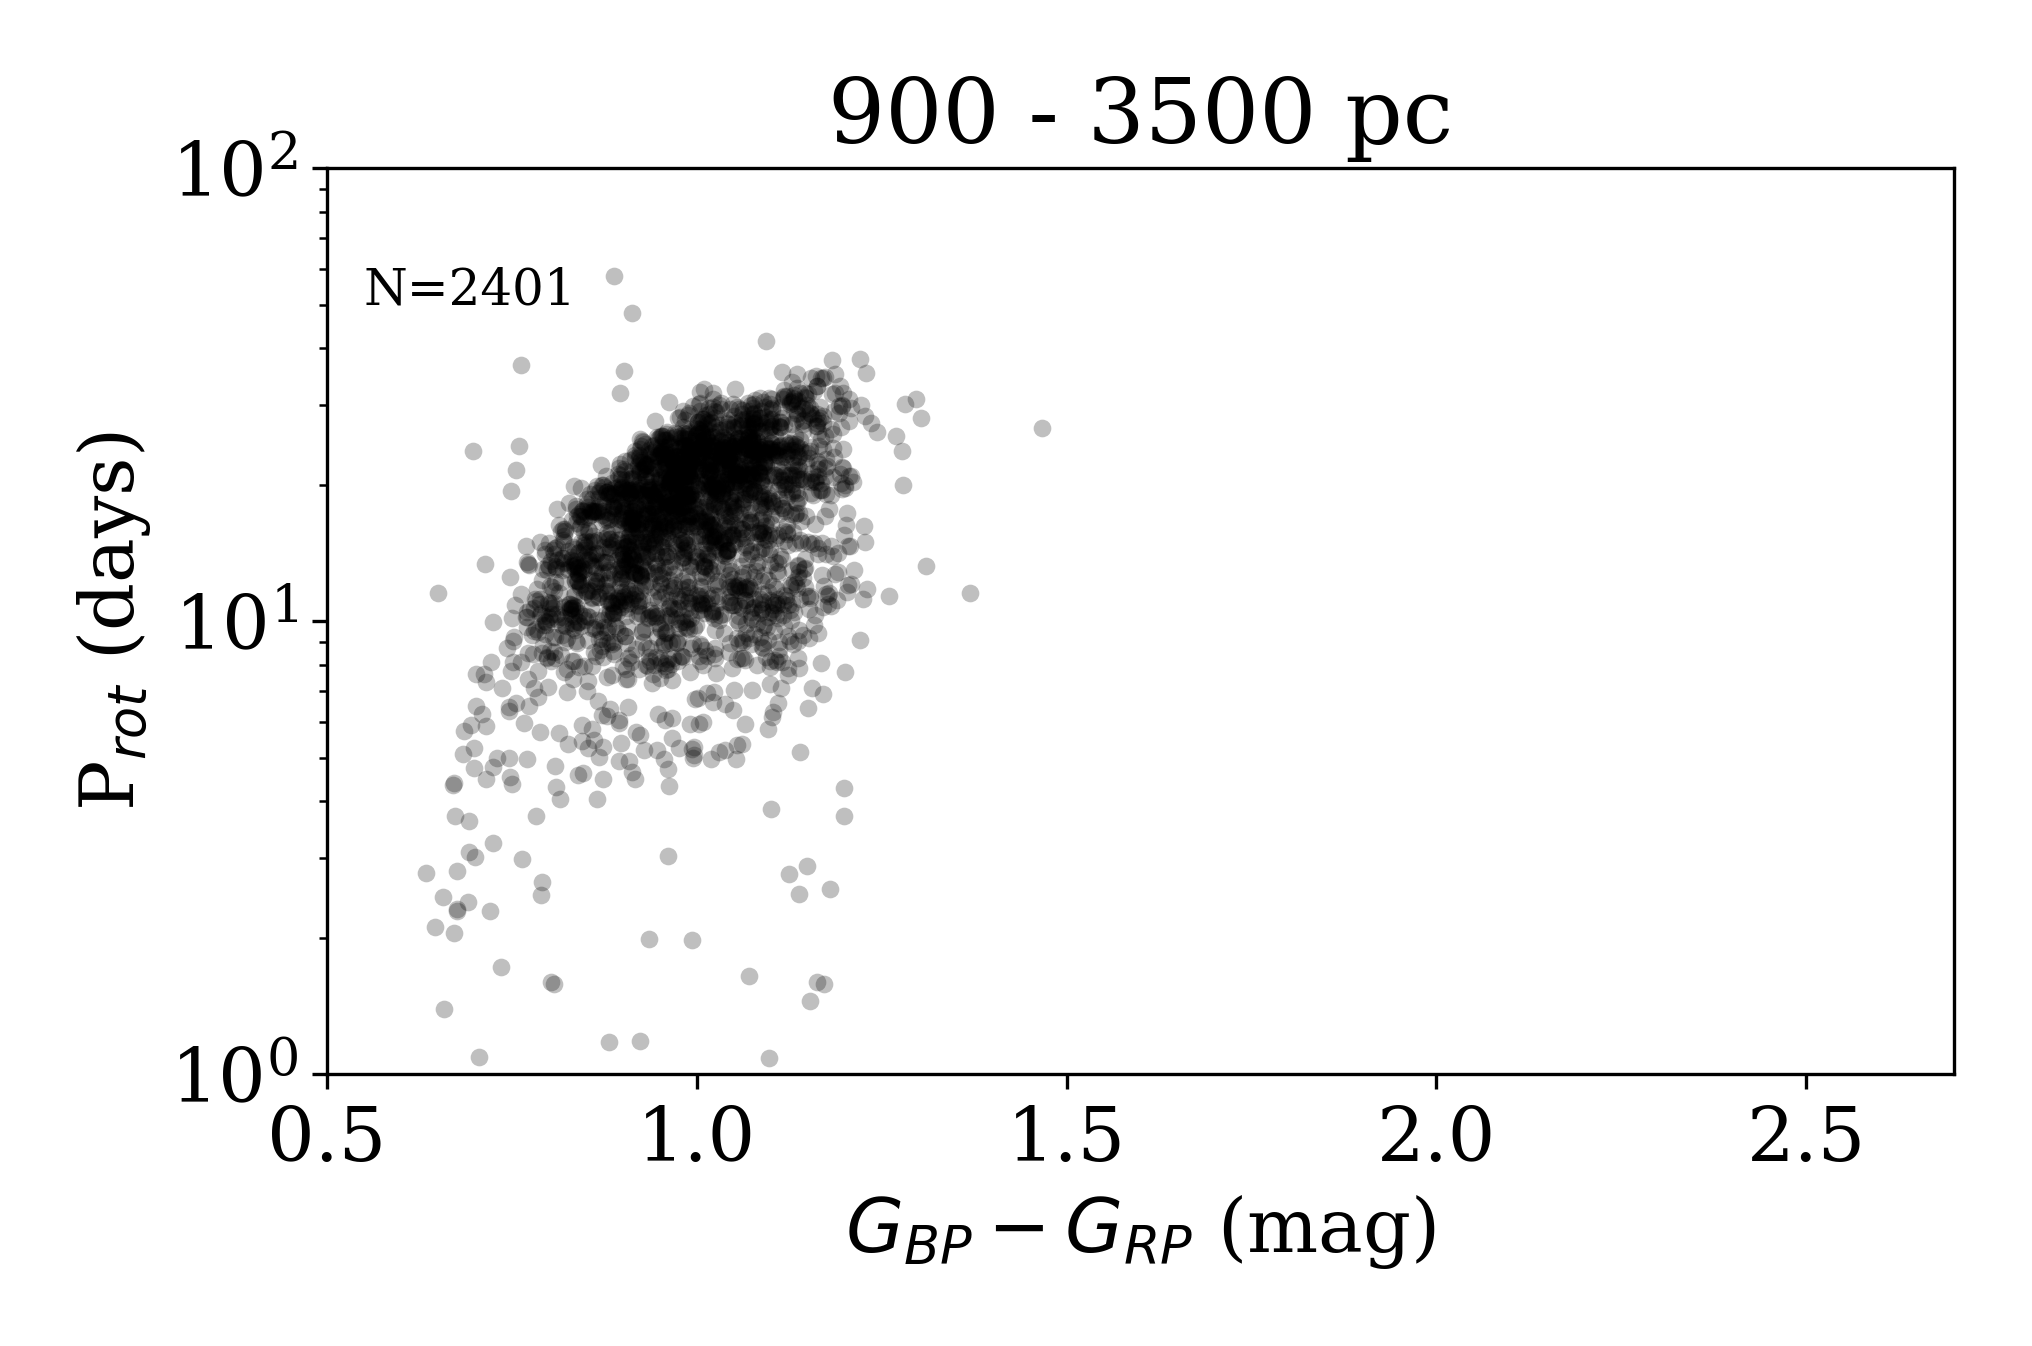
\includegraphics[width=3.5in]{../figures/rot_dist_900}
\caption{Color--period diagrams for our sample of likely main sequence stars, divided into bins of distance. Our nearest bin (within 350pc) is effectively the distance analyzed in \citet{davenport2017} using Gaia DR1, and clearly shows the rotation period bimodality for the entire sample. The brighter magnitude limit of the \Kepler sample results in redder (fainter) stars missing in our further distance bins. The rotation period bimodality can be seen in the 350-525 pc bin, but is not found in the bluer stars at further distances.
}
\label{fig:color_period}
\end{figure*}



%\begin{figure}[]
%\centering
%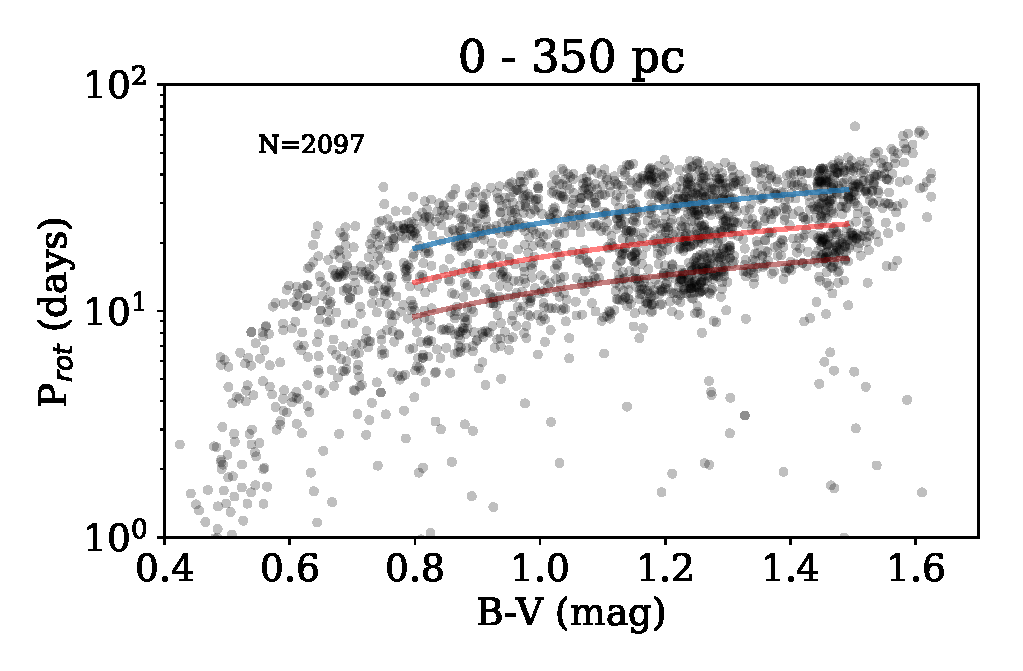
\includegraphics[width=3.5in]{../figures/B_V_rot}
%\caption{converted to B-V using Padova isochrone colors. 3 gyrochrones from \citet{meibom2009} with ages 300 Myr (dark red), 600 Myr (bright red), and 1.2 Gyr (blue) are shown.
%}
%%\label{fig:cmd}
%\end{figure}
%

\begin{figure}[]
\centering
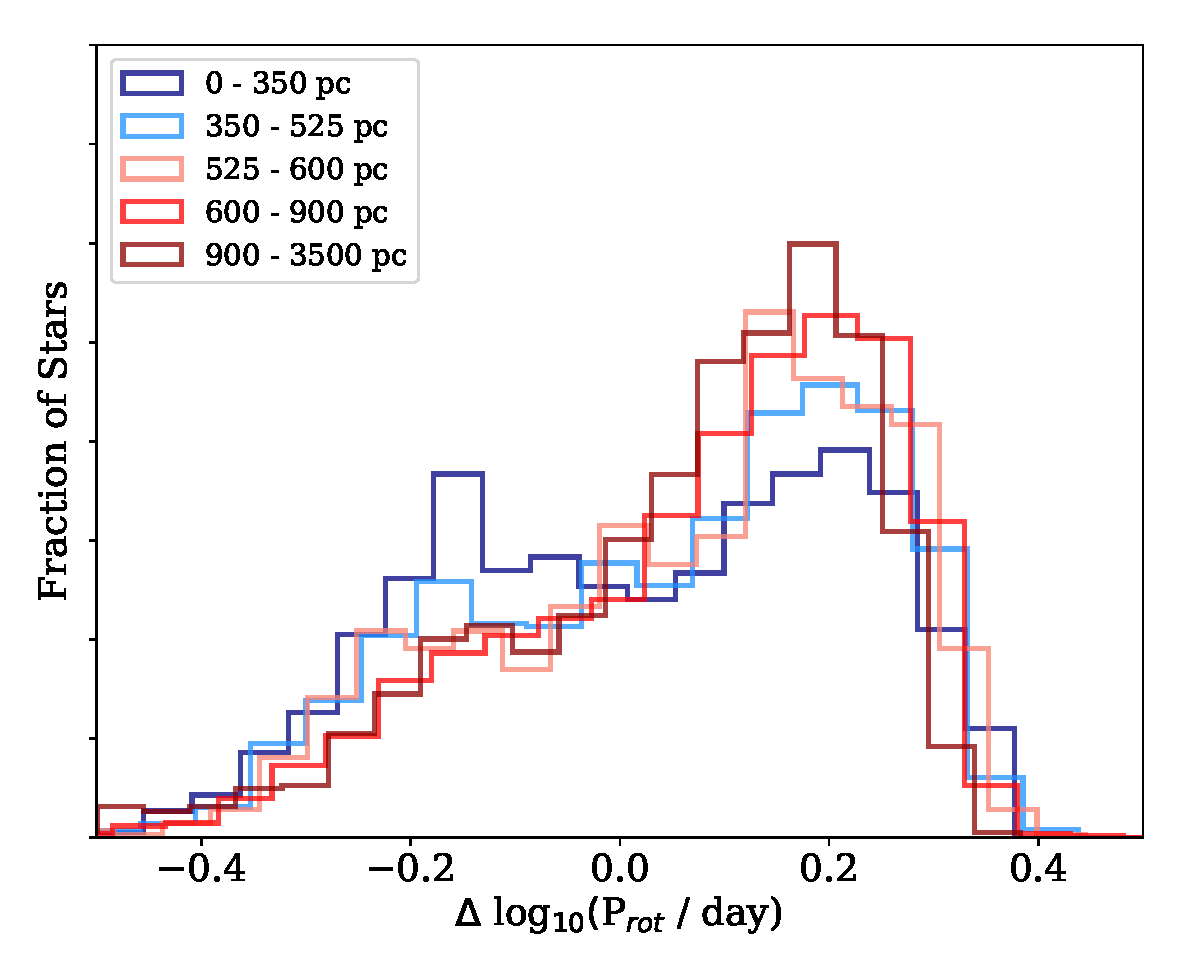
\includegraphics[width=3.5in]{../figures/delta_per}
\caption{Histograms of the log rotation periods after a 600 Myr gyrochrone was subtracted for stars in the same five distance bins shown in Figure \ref{fig:color_period}.
}
\label{fig:per_hist}
\end{figure}





\begin{figure*}[]
\centering
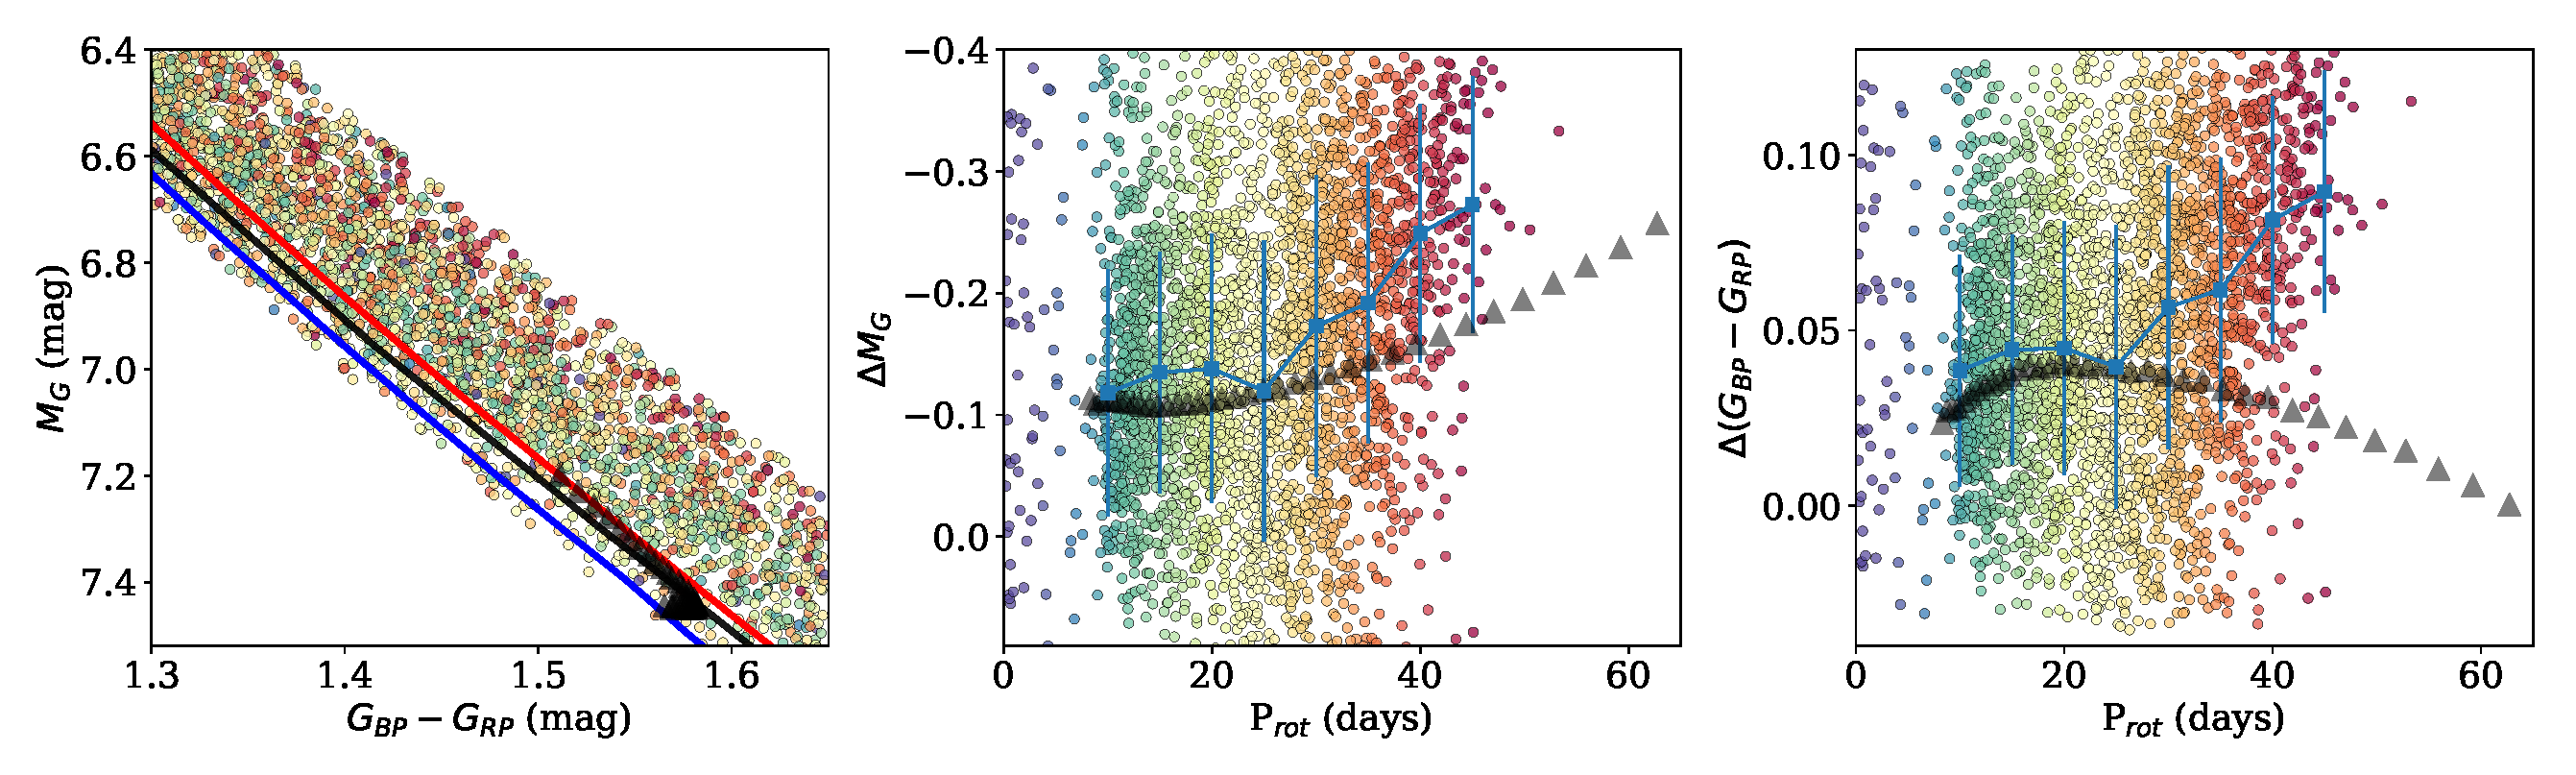
\includegraphics[width=6.5in]{../figures/cmd_zoom}
\caption{
}
\label{fig:cmd_zoom}
\end{figure*}




%\begin{figure}[]
%\centering
%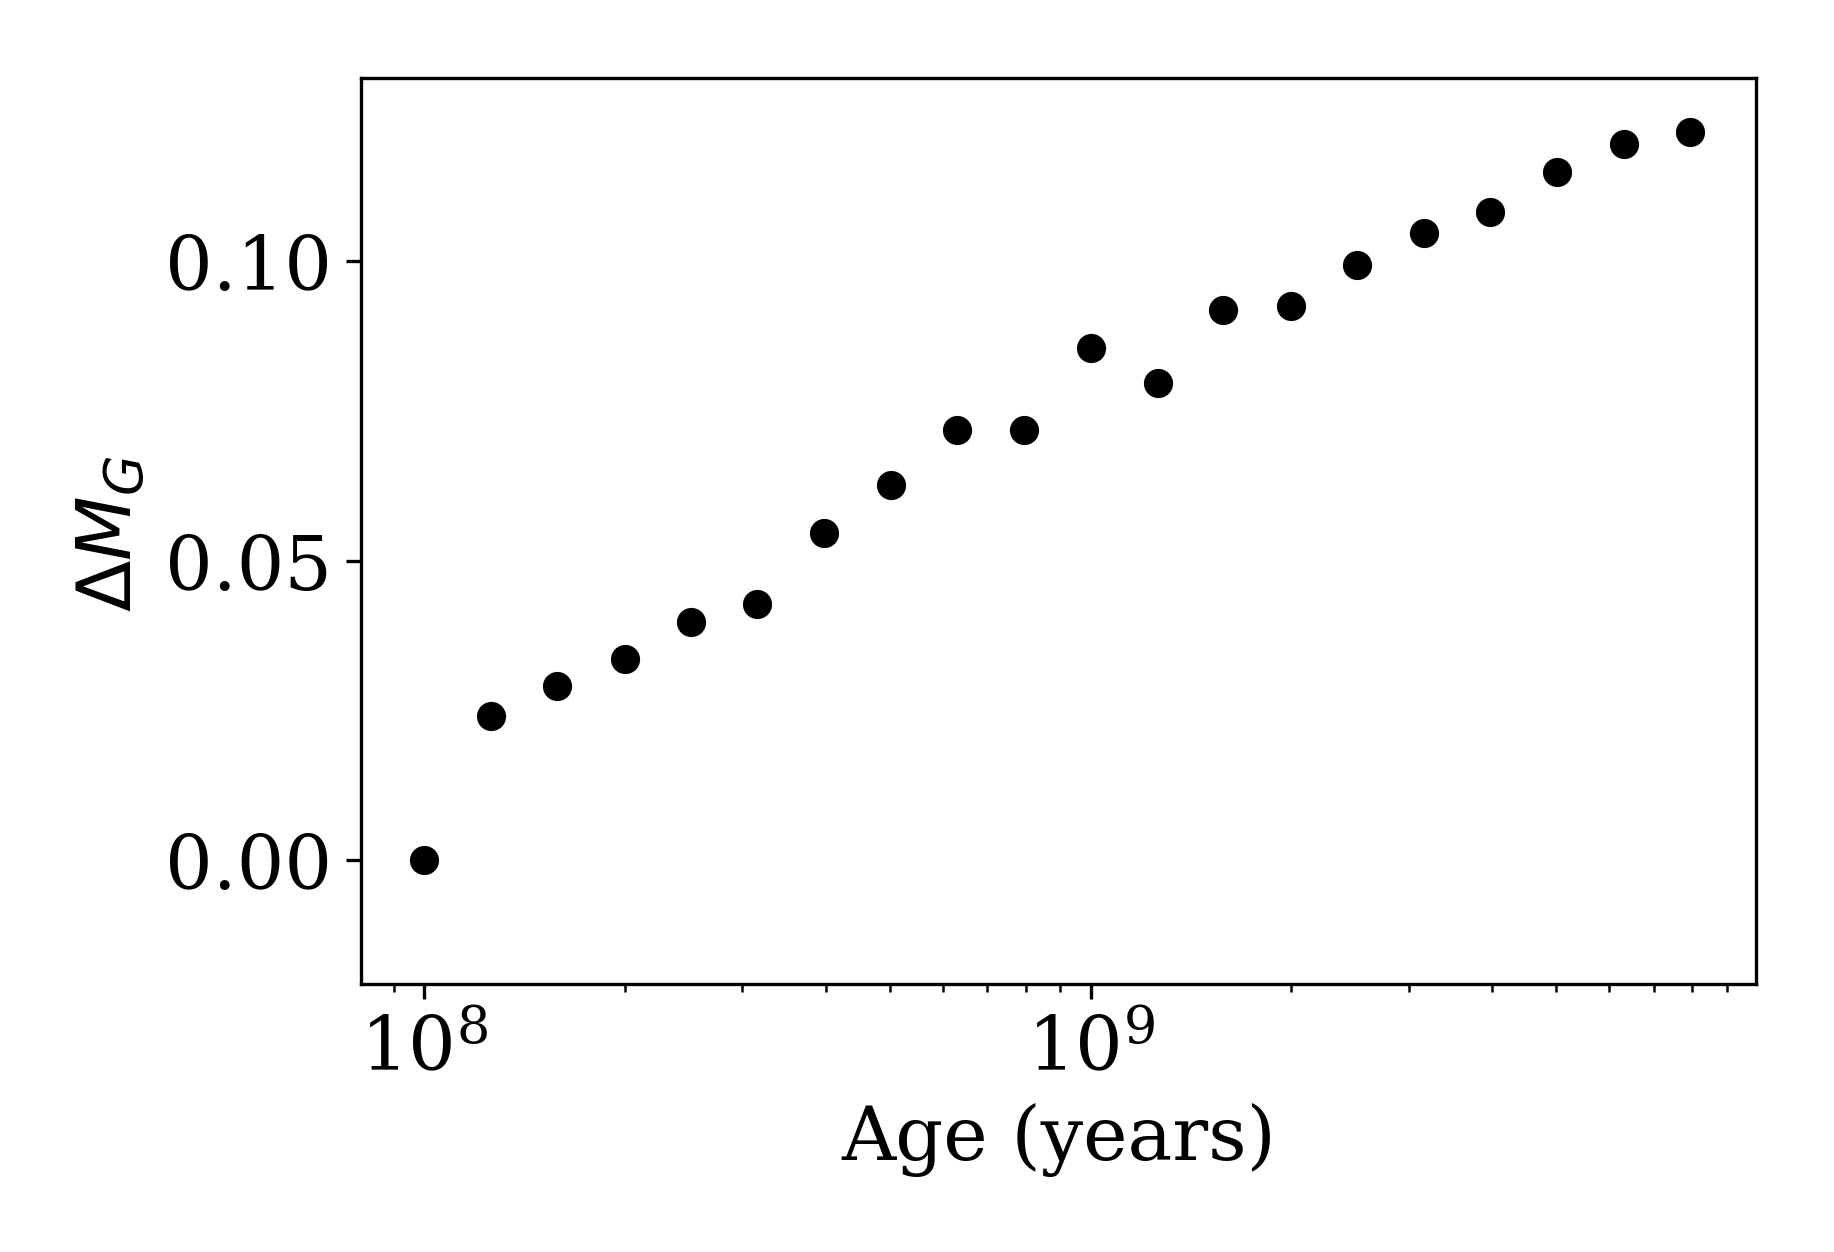
\includegraphics[width=3.5in]{../figures/iso_age}
%\caption{
%}
%%\label{fig:cmd}
%\end{figure}



%%%%%%%%%%%%%%%%%%%%%%
\section{Discussion}
%
%Using a combination of data from \Kepler and Gaia DR1, I have explored the rotation period distribution for 440 nearby main sequence stars. A bimodal rotation period distribution has been found in stars with temperatures ranging from 5000 K to 6500 K. This feature matches that found in cooler stars from \Kepler, but was only revealed thanks to the enhanced ability to distinguish dwarfs from subgiants using Gaia data. 
%A tenuous difference in the TGAS total proper motion for stars in the fast and slow rotating groups is found, which is in agreement with the findings for cool stars by \citet{mcquillan2013}.
%
%While a definitive explanation for this period bimodality has not been reached, the findings to date seem to favor stellar ages as the cause. In this scenario the star formation history for nearby stars would be dominated by two epochs of star formation, one short event centered at a few hundred Myr, and one long event centered at a few Gyr (slightly younger than the Sun). It is also worth noting that the space volume probed by the TGAS sample investigated here is very similar to that covered by the temperature-selected cool star sample in \citet{mcquillan2013}. The median parallax distance for stars in this work is 285 pc, while the median isochrone distance for the K and M dwarfs is $\sim$216 pc. This points to the period distribution being a localized age artifact. 
%Determining how localized this age distribution is, and if it can be confirmed for stars across the HR diagram including giants, is a key goal for future Gaia data releases.
%
%
%The period bimodality may yet be a manifestation of the ``Vaughan-Preston'' gap observed in chromospheric activity indicators from solar type stars. Such a feature has also been discussed for rotating stars by \citet{kado-fong2016}. Given that the mass range for the bimodality explored here and in \citet{mcquillan2014} covers stars with solar-type dynamos (those having a tachocline, late F through early M) such a model cannot be fully ruled out at this time. Though there have been many rotation studies for cool stars \citep[e.g.][]{irwin2011,newton2016,stelzer2016} too few rotation periods have been measured for stars across the ``fully convective boundary'' ($T_{eff}<3000$ K, spectral type $\sim$M4) to tell if the bimodal period feature continues to cooler temperatures, which would support the age distribution model. 
%If the bimodality is due to stars crossing a phase of rapid angular momentum evolution, we would expect to see it in stellar clusters at or near the critical age. The lack of this feature in the clusters observed to date could be due to no cluster being close enough to the critical age, which the gyrochrone in Figure \ref{fig:gyro} shows is near 600 Myr. Further studies of rotation periods for stars in intermediate age open clusters (e.g. the Hyades) may help solve this mystery \citep[e.g.][]{douglas2014}.
%
%Finally, this exploratory work has highlighted the utility of using astrometric data from Gaia combined with detailed light curve statistics from \Kepler to reveal hidden substructure in the properties of field stars. Looking forward to the astrometric precision of future Gaia data releases, this combination will be effective at separating dwarf stars from subgiants for nearly the entire \Kepler and K2 databases, and enable accurate age maps for field stars.



%%%%%%%%%%%%%%%%%
\acknowledgments

JRAD is supported by an NSF Astronomy and Astrophysics Postdoctoral Fellowship under award AST-1501418. 

This work made use of the \url{gaia-kepler.fun} crossmatch database created by Megan Bedell.

This project was developed as part of the 2018 NYC Gaia Sprint, hosted by the Center for Computational Astrophysics at the Simons Foundation in New York City.

%This research made use of the cross-match service, and the SIMBAD database, provided by CDS, Strasbourg, France.
%
%This work has made use of data from the European Space Agency (ESA)
%mission {\it Gaia} (\url{http://www.cosmos.esa.int/gaia}), processed by
%the {\it Gaia} Data Processing and Analysis Consortium (DPAC,
%\url{http://www.cosmos.esa.int/web/gaia/dpac/consortium}). Funding
%for the DPAC has been provided by national institutions, in particular
%the institutions participating in the {\it Gaia} Multilateral Agreement.




\bibliography{/Users/james/Dropbox/references}

\end{document}
